\documentclass[11pt,a4paper]{article}

%
% $Id: userguide.tex 526 2007-10-31 08:57:09Z schnelle $
%

\usepackage[latin1]{inputenc}
\usepackage{graphics}
\usepackage{graphicx}
\usepackage{url}
\usepackage{listings}
\usepackage{xcolor}
\usepackage{jvoicexml}

\title{JVoiceXML Vendor Guide}
\version{0.1}
\author{Dr. Dirk Schnelle-Walka}
\email{dirk.schnelle@jvoicexml.org}
\date{\today}

\begin{document}
\pagestyle{empty}
\lstset{language=Java,language=XML,
        backgroundcolor=\color{lightgray},
        basicstyle=\small,
        numbers=left,
        numberstyle=\tiny,
        stepnumber=5}

\maketitle

\pagestyle{headings}

\tableofcontents

\newpage

\begin{abstract}
This documents describes the API of JVoiceXML from the vendor's point of
view. It provides information about how to hook your custom implementation
platform into the JVoiceXML voice browser.
\end{abstract}


\section{Introduction}
\label{sec:introduction}

JVoiceXML is a free VoiceXML~\cite{w3.org:voicexml} implementation written in 
the JAVA programming language. It offers a library for easy VoiceXML
document creation and a VoiceXML interpreter to process 
VoiceXML documents using JAVA standard APIs such as JSAPI~\cite{sun:jsapi} and
JTAPI~\cite{sun:jsapi}.

VoiceXML is hosted at SourceForge~\cite{sourceforge} as an open source project.
You find everything that is related to this project under
\url{http://sourceforge.net/projects/jvoicexml/}.
The work on the browser is still in progress and not all tags are
supported. You are invited to help us finishing the work to make this
project a success.

This document provides information on how to hook your custom implemenation
paltform into the JVoiceXML voice browser. It is assumed that readers are
familiar with the concepts of VoiceXML and Java programming.

This document refers to UNIX and Windows systems. JVoiceXML will work with 
any other operating systems that support Java 5, too.

Nobody is perfect, so you may find some errors or small things to correct.
Please let me know if you think you found something that should be written
differently or should be added.

\section{Architectural Overview}
\label{sec:arch-overv}

Before going into detail the general architecture and concepts are presented.
The basic architecture is shown in figure~\ref{fig:main-components}.
\begin{figure}
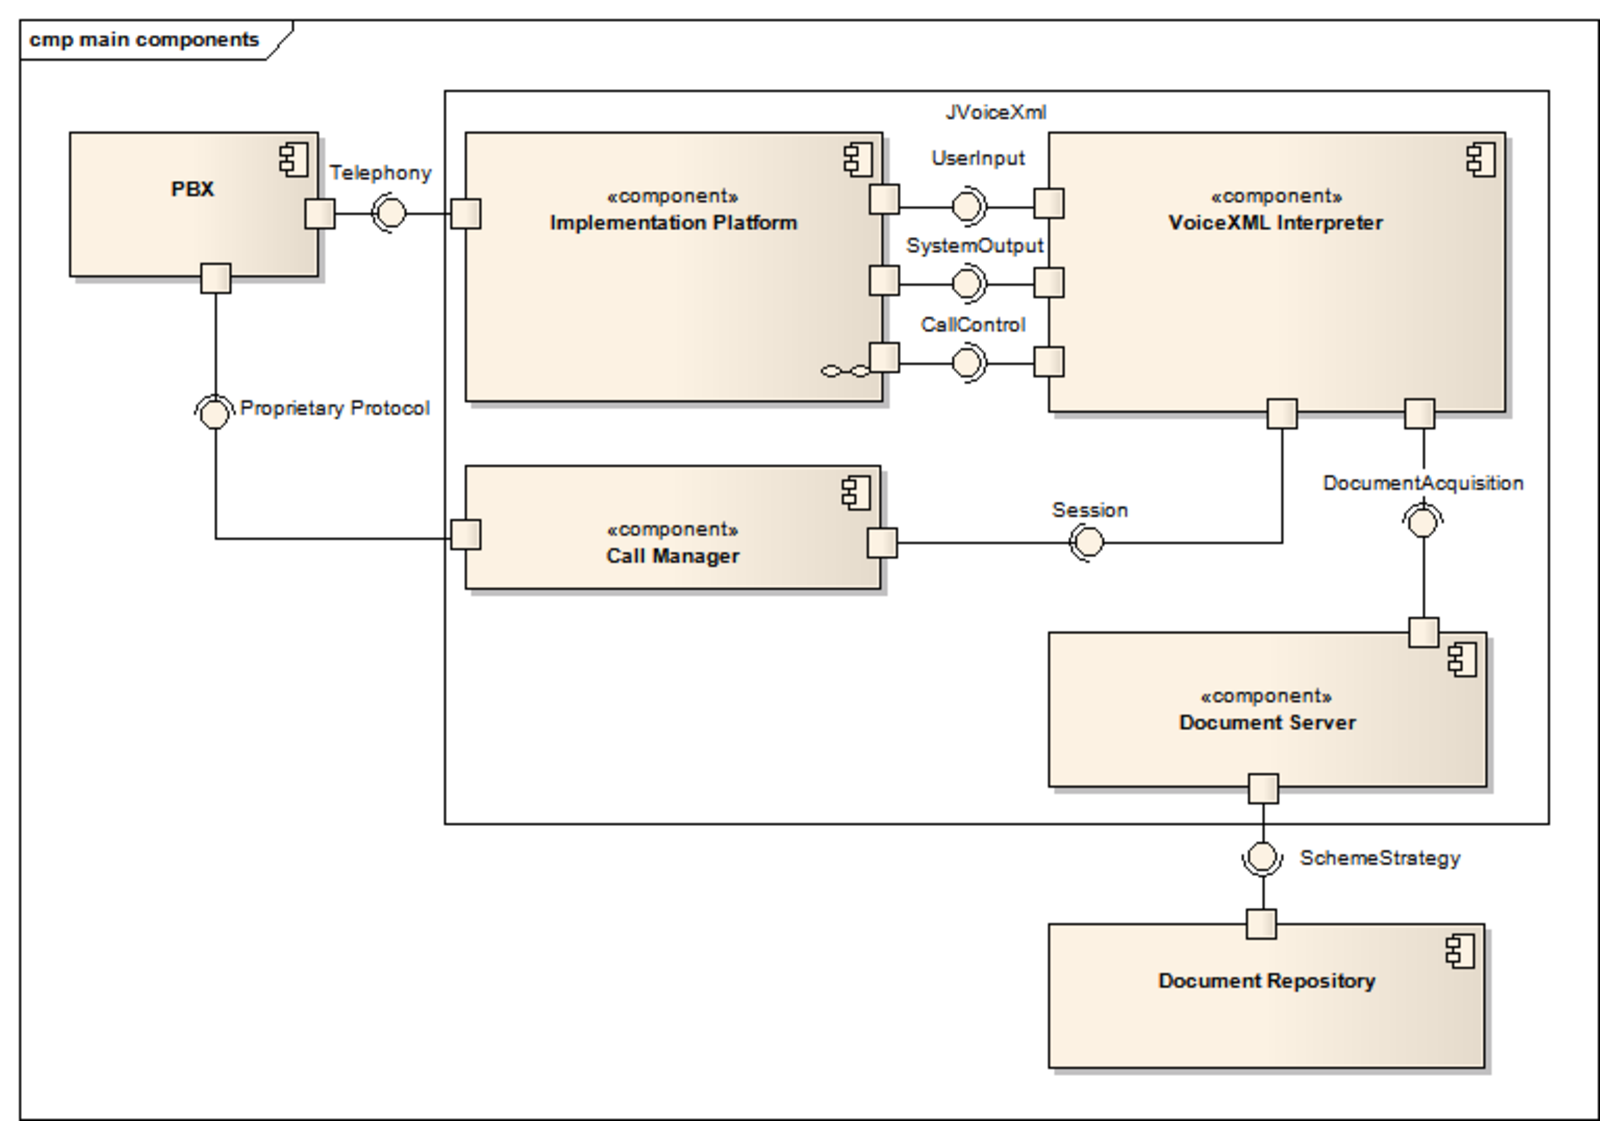
\includegraphics[width=\linewidth]{cd-main-components}
\caption{Basic architecture of JVoiceXML}
\label{fig:main-components}
\end{figure}
The point of interest is the \emph{Implemtation Platform}.
Figure~\ref{fig:implementationplatform} shows the composite parts of that
component.
\begin{figure}
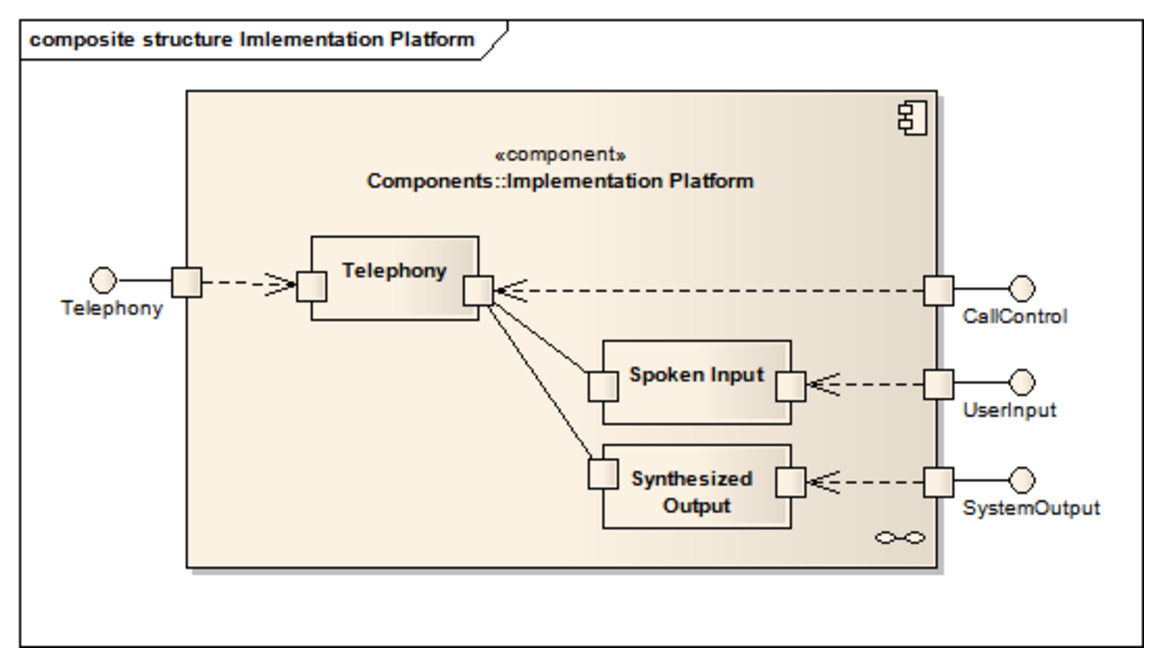
\includegraphics[width=\linewidth]{csd-implementation-platform}
\caption{Compositite parts of the implementation platform}
\label{fig:implementationplatform}
\end{figure}

\section{Steps to your own implementation platform}

\end{document}
